\documentclass[11pt]{article}
\usepackage[textwidth=18.0cm, textheight=23.0cm, top=2.0cm]{geometry}
\usepackage{pst-all}
\usepackage{amssymb}
\usepackage{tikz}
\usepackage{underscore}\begin{document}
\pagestyle{empty}


ClassName: \underline{\textbf{Class_08.2bp-19}}
\par
BinSize: \underline{\textbf{100 × 100}}
\par
ReduceSize: \underline{\textbf{100 × 100}}
\par
TypeNum: \underline{\textbf{40}}
\par
Num: \underline{\textbf{40}}
\par
OutS: \underline{\textbf{130000}}
\par
InS: \underline{\textbf{105358}}
\par
Rate: \underline{\textbf{0.810}}
\par
UB: \underline{\textbf{13}}
\par
LB0: \underline{\textbf{13}}
\par
LB: \underline{\textbf{13}}
\par
LBWithCut: \underline{\textbf{13}}
\par
NodeCut: \underline{\textbf{0}}
\par
ExtendedNodeCnt: \underline{\textbf{1}}
\par
GenNodeCnt: \underline{\textbf{1}}
\par
PrimalNode: \underline{\textbf{0}}
\par
ColumnCount: \underline{\textbf{13}}
\par
TotalCutCount: \underline{\textbf{0}}
\par
RootCutCount: \underline{\textbf{0}}
\par
LPSolverCnt: \underline{\textbf{1}}
\par
PricingSolverCnt: \underline{\textbf{0}}
\par
BranchAndBoundNum: \underline{\textbf{1}}
\par
isOpt: \underline{\textbf{true}}
\par
TimeOnInitSolution: \underline{\textbf{600.000 s}}
\par
TimeOnPrimal: \underline{\textbf{0.000 s}}
\par
TimeOnPricing: \underline{\textbf{0.000 s}}
\par
TimeOnRmp: \underline{\textbf{0.058 s}}
\par
TotalTime: \underline{\textbf{600.325 s}}
\par
\newpage


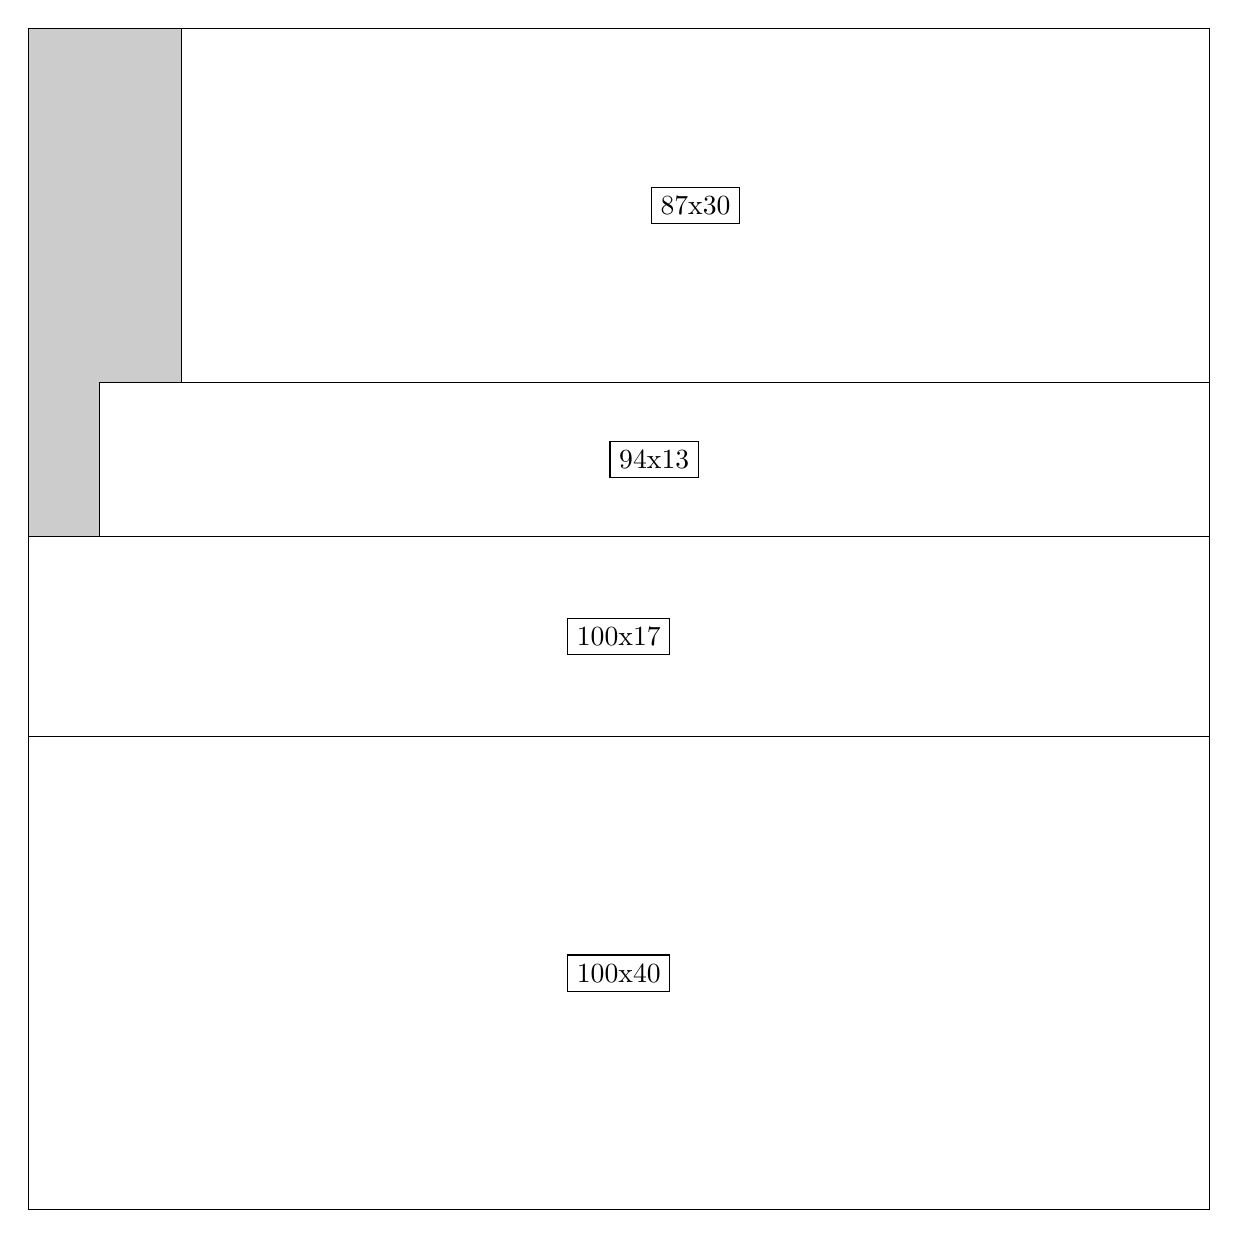
\begin{tikzpicture}[shorten >=1pt,scale=1.0,every node/.style={scale=1.0},->]
\tikzstyle{vertex}=[circle,fill=black!25,minimum size=14pt,inner sep=0pt]
\filldraw[fill=gray!40!white, draw=black] (0,0) rectangle (15.0,15.0);
\foreach \name/\x/\y/\w/\h in {100x40/0.0/0.0/15.0/6.0,100x17/0.0/6.0/15.0/2.55,94x13/0.8999999999999999/8.549999999999999/14.1/1.95,87x30/1.95/10.5/13.049999999999999/4.5}
\filldraw[fill=white!40!white, draw=black] (\x,\y) rectangle node[draw] (\name) {\name} ++(\w,\h);
\end{tikzpicture}


w =100 , h =40 , x =0 , y =0 , v =4000
\par
w =100 , h =17 , x =0 , y =40 , v =1700
\par
w =94 , h =13 , x =6 , y =57 , v =1222
\par
w =87 , h =30 , x =13 , y =70 , v =2610
\par
\newpage


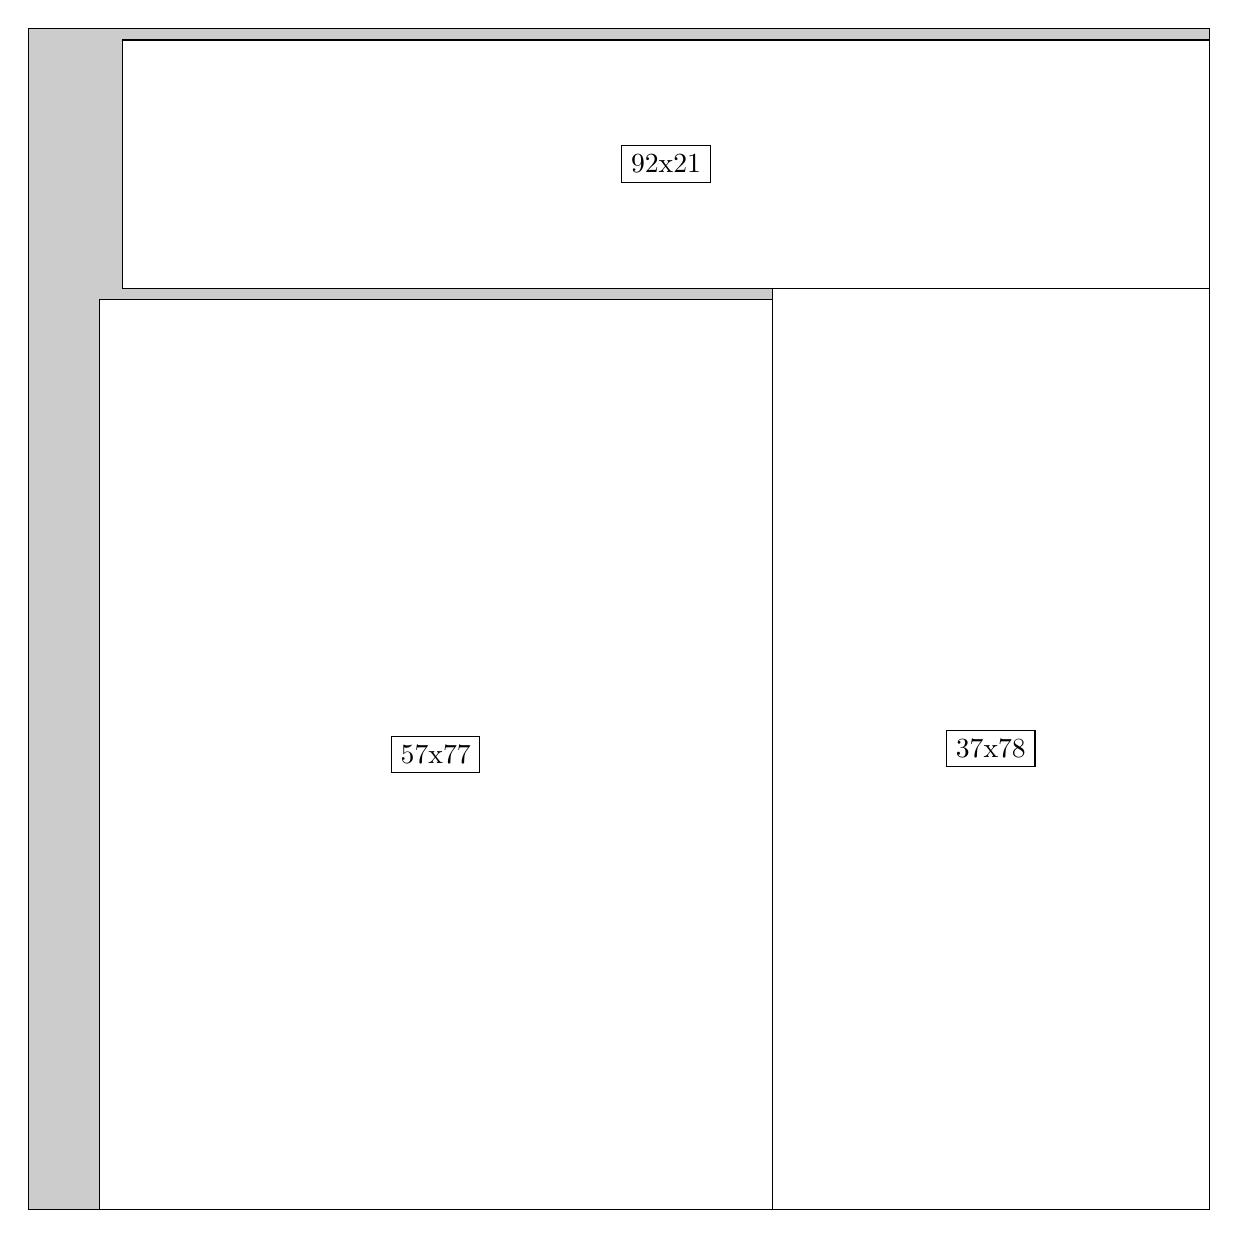
\begin{tikzpicture}[shorten >=1pt,scale=1.0,every node/.style={scale=1.0},->]
\tikzstyle{vertex}=[circle,fill=black!25,minimum size=14pt,inner sep=0pt]
\filldraw[fill=gray!40!white, draw=black] (0,0) rectangle (15.0,15.0);
\foreach \name/\x/\y/\w/\h in {37x78/9.45/0.0/5.55/11.7,57x77/0.8999999999999999/0.0/8.549999999999999/11.549999999999999,92x21/1.2/11.7/13.799999999999999/3.15}
\filldraw[fill=white!40!white, draw=black] (\x,\y) rectangle node[draw] (\name) {\name} ++(\w,\h);
\end{tikzpicture}


w =37 , h =78 , x =63 , y =0 , v =2886
\par
w =57 , h =77 , x =6 , y =0 , v =4389
\par
w =92 , h =21 , x =8 , y =78 , v =1932
\par
\newpage


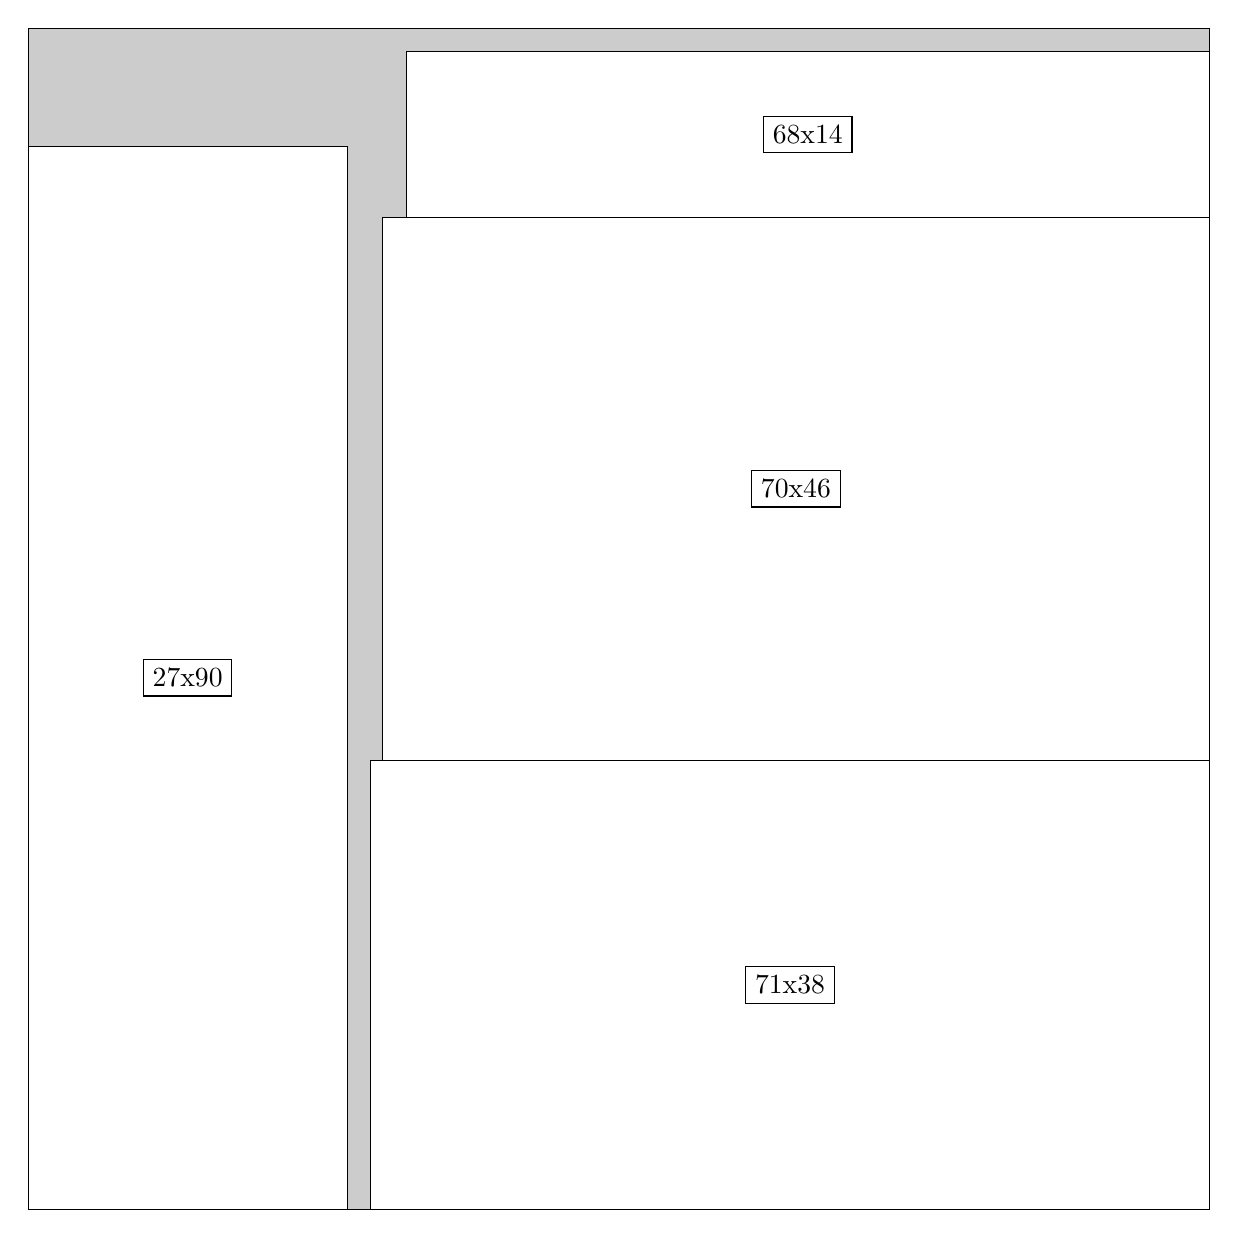
\begin{tikzpicture}[shorten >=1pt,scale=1.0,every node/.style={scale=1.0},->]
\tikzstyle{vertex}=[circle,fill=black!25,minimum size=14pt,inner sep=0pt]
\filldraw[fill=gray!40!white, draw=black] (0,0) rectangle (15.0,15.0);
\foreach \name/\x/\y/\w/\h in {71x38/4.35/0.0/10.65/5.7,70x46/4.5/5.7/10.5/6.8999999999999995,68x14/4.8/12.6/10.2/2.1,27x90/0.0/0.0/4.05/13.5}
\filldraw[fill=white!40!white, draw=black] (\x,\y) rectangle node[draw] (\name) {\name} ++(\w,\h);
\end{tikzpicture}


w =71 , h =38 , x =29 , y =0 , v =2698
\par
w =70 , h =46 , x =30 , y =38 , v =3220
\par
w =68 , h =14 , x =32 , y =84 , v =952
\par
w =27 , h =90 , x =0 , y =0 , v =2430
\par
\newpage


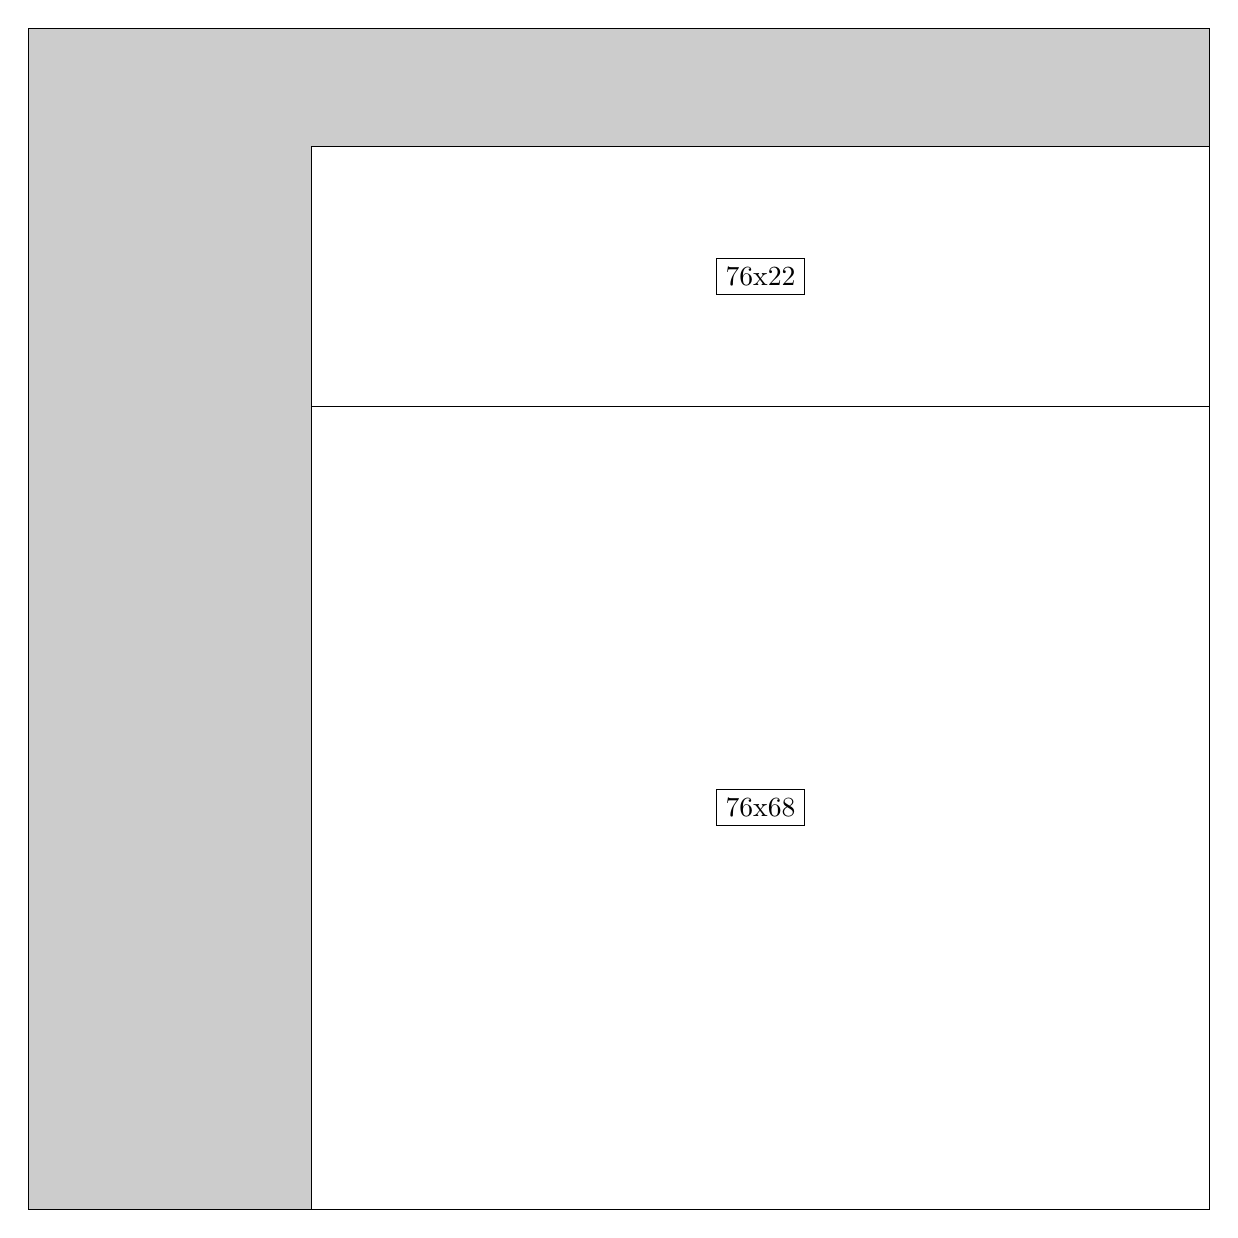
\begin{tikzpicture}[shorten >=1pt,scale=1.0,every node/.style={scale=1.0},->]
\tikzstyle{vertex}=[circle,fill=black!25,minimum size=14pt,inner sep=0pt]
\filldraw[fill=gray!40!white, draw=black] (0,0) rectangle (15.0,15.0);
\foreach \name/\x/\y/\w/\h in {76x68/3.5999999999999996/0.0/11.4/10.2,76x22/3.5999999999999996/10.2/11.4/3.3}
\filldraw[fill=white!40!white, draw=black] (\x,\y) rectangle node[draw] (\name) {\name} ++(\w,\h);
\end{tikzpicture}


w =76 , h =68 , x =24 , y =0 , v =5168
\par
w =76 , h =22 , x =24 , y =68 , v =1672
\par
\newpage


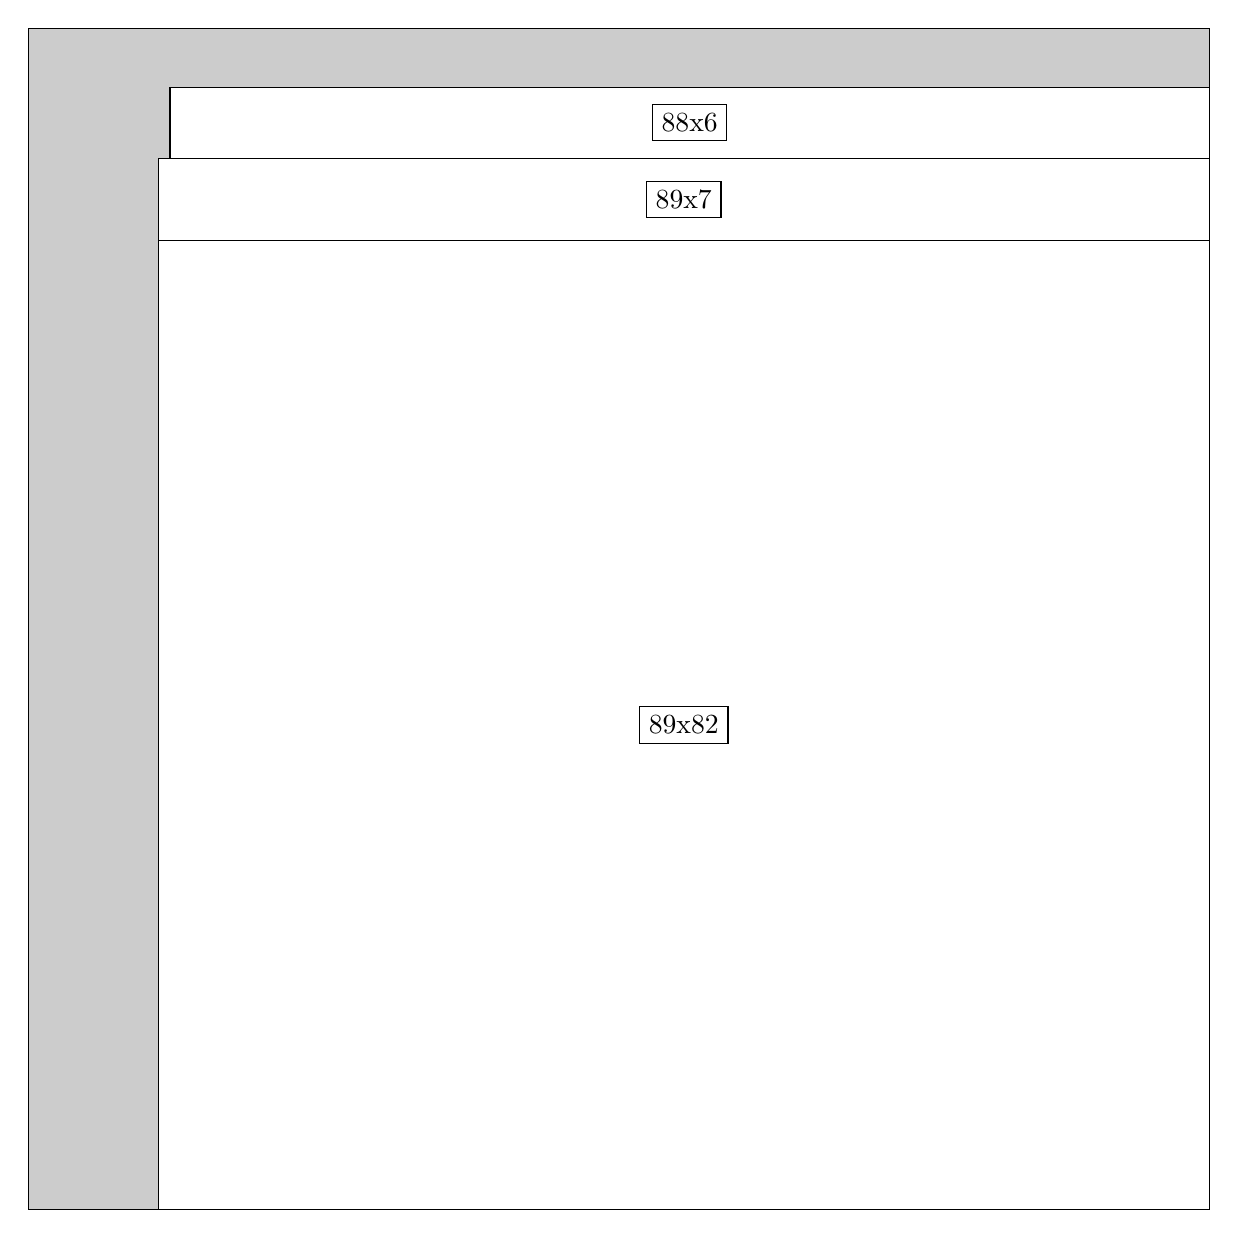
\begin{tikzpicture}[shorten >=1pt,scale=1.0,every node/.style={scale=1.0},->]
\tikzstyle{vertex}=[circle,fill=black!25,minimum size=14pt,inner sep=0pt]
\filldraw[fill=gray!40!white, draw=black] (0,0) rectangle (15.0,15.0);
\foreach \name/\x/\y/\w/\h in {89x82/1.65/0.0/13.35/12.299999999999999,89x7/1.65/12.299999999999999/13.35/1.05,88x6/1.7999999999999998/13.35/13.2/0.8999999999999999}
\filldraw[fill=white!40!white, draw=black] (\x,\y) rectangle node[draw] (\name) {\name} ++(\w,\h);
\end{tikzpicture}


w =89 , h =82 , x =11 , y =0 , v =7298
\par
w =89 , h =7 , x =11 , y =82 , v =623
\par
w =88 , h =6 , x =12 , y =89 , v =528
\par
\newpage


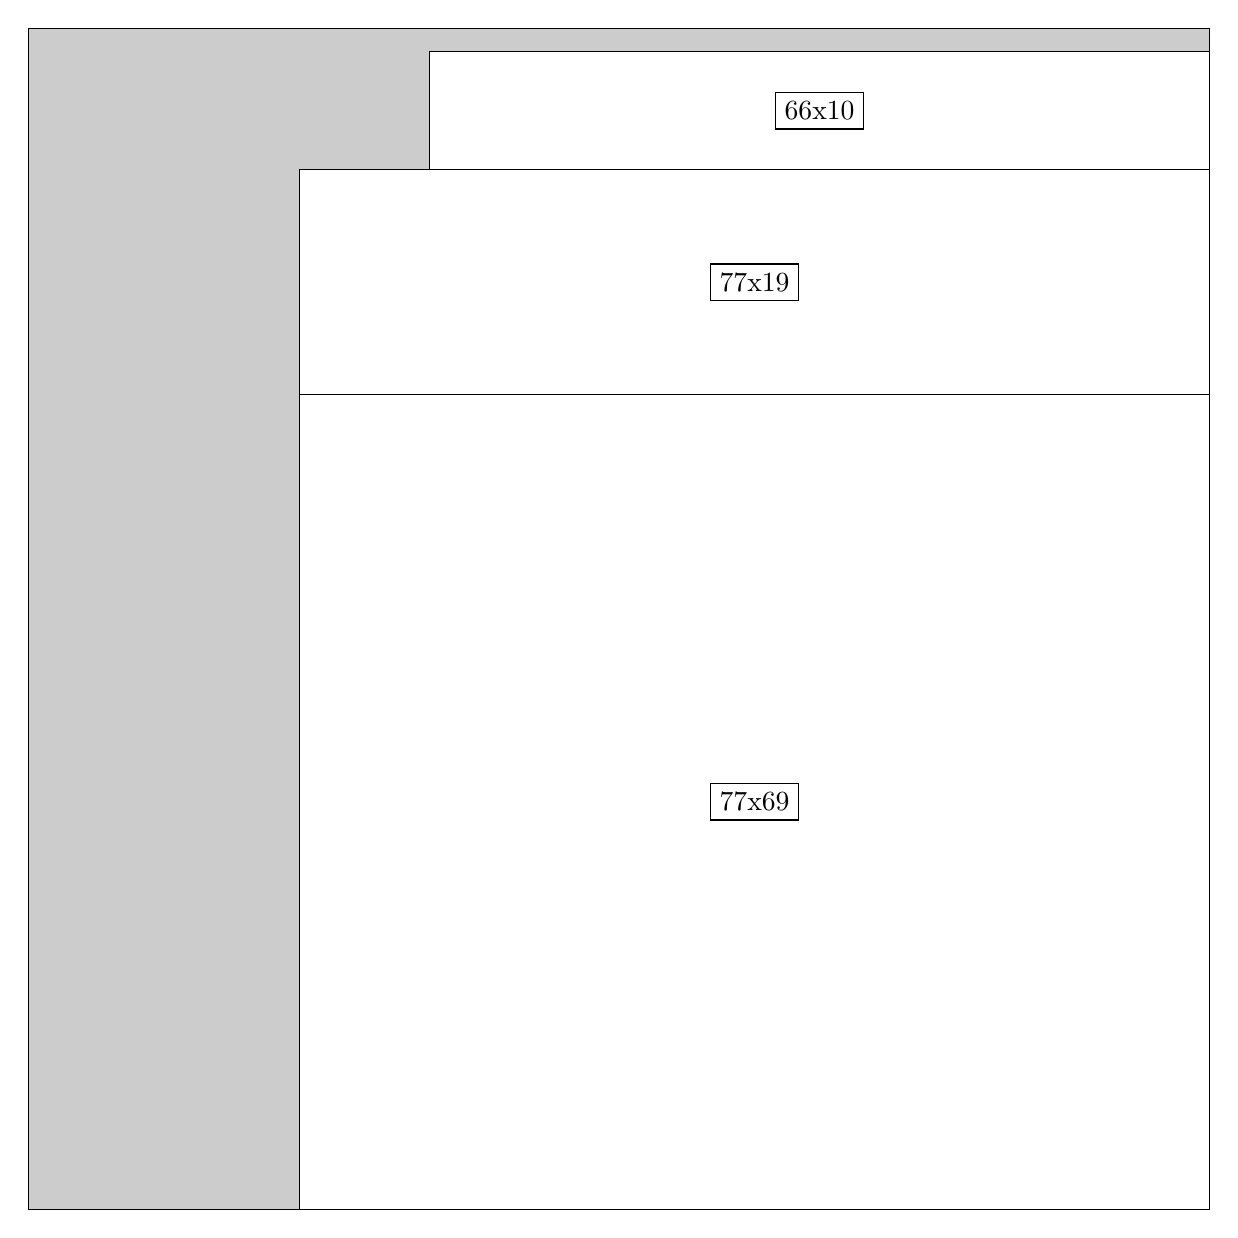
\begin{tikzpicture}[shorten >=1pt,scale=1.0,every node/.style={scale=1.0},->]
\tikzstyle{vertex}=[circle,fill=black!25,minimum size=14pt,inner sep=0pt]
\filldraw[fill=gray!40!white, draw=black] (0,0) rectangle (15.0,15.0);
\foreach \name/\x/\y/\w/\h in {77x69/3.4499999999999997/0.0/11.549999999999999/10.35,77x19/3.4499999999999997/10.35/11.549999999999999/2.85,66x10/5.1/13.2/9.9/1.5}
\filldraw[fill=white!40!white, draw=black] (\x,\y) rectangle node[draw] (\name) {\name} ++(\w,\h);
\end{tikzpicture}


w =77 , h =69 , x =23 , y =0 , v =5313
\par
w =77 , h =19 , x =23 , y =69 , v =1463
\par
w =66 , h =10 , x =34 , y =88 , v =660
\par
\newpage


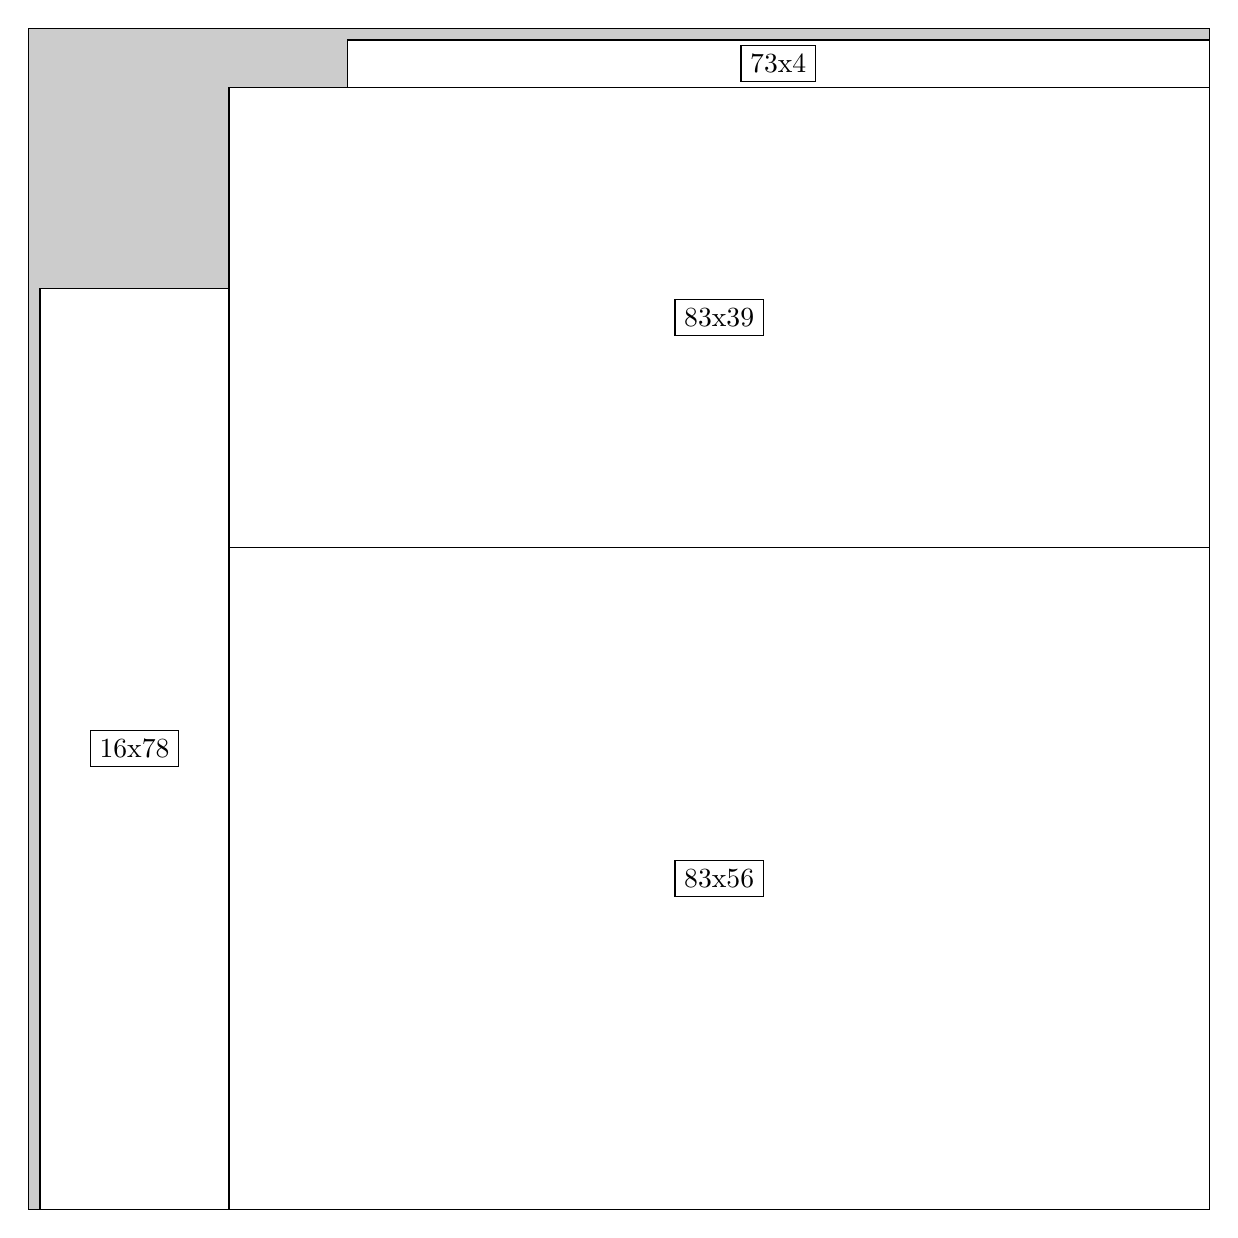
\begin{tikzpicture}[shorten >=1pt,scale=1.0,every node/.style={scale=1.0},->]
\tikzstyle{vertex}=[circle,fill=black!25,minimum size=14pt,inner sep=0pt]
\filldraw[fill=gray!40!white, draw=black] (0,0) rectangle (15.0,15.0);
\foreach \name/\x/\y/\w/\h in {83x56/2.55/0.0/12.45/8.4,83x39/2.55/8.4/12.45/5.85,73x4/4.05/14.25/10.95/0.6,16x78/0.15/0.0/2.4/11.7}
\filldraw[fill=white!40!white, draw=black] (\x,\y) rectangle node[draw] (\name) {\name} ++(\w,\h);
\end{tikzpicture}


w =83 , h =56 , x =17 , y =0 , v =4648
\par
w =83 , h =39 , x =17 , y =56 , v =3237
\par
w =73 , h =4 , x =27 , y =95 , v =292
\par
w =16 , h =78 , x =1 , y =0 , v =1248
\par
\newpage


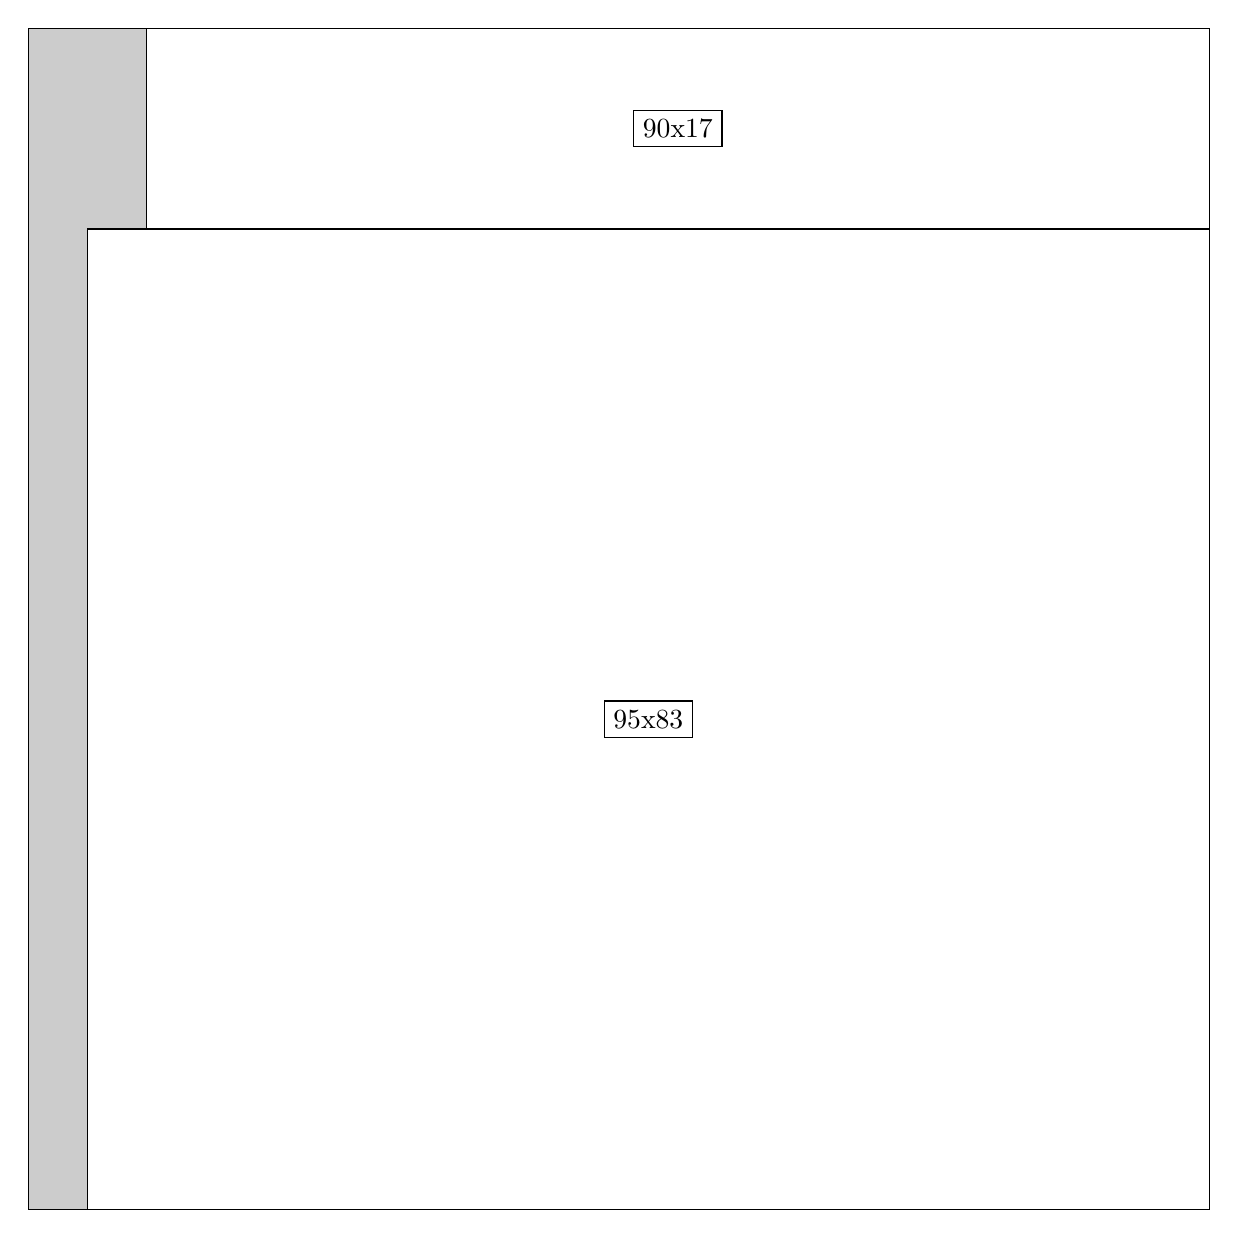
\begin{tikzpicture}[shorten >=1pt,scale=1.0,every node/.style={scale=1.0},->]
\tikzstyle{vertex}=[circle,fill=black!25,minimum size=14pt,inner sep=0pt]
\filldraw[fill=gray!40!white, draw=black] (0,0) rectangle (15.0,15.0);
\foreach \name/\x/\y/\w/\h in {95x83/0.75/0.0/14.25/12.45,90x17/1.5/12.45/13.5/2.55}
\filldraw[fill=white!40!white, draw=black] (\x,\y) rectangle node[draw] (\name) {\name} ++(\w,\h);
\end{tikzpicture}


w =95 , h =83 , x =5 , y =0 , v =7885
\par
w =90 , h =17 , x =10 , y =83 , v =1530
\par
\newpage


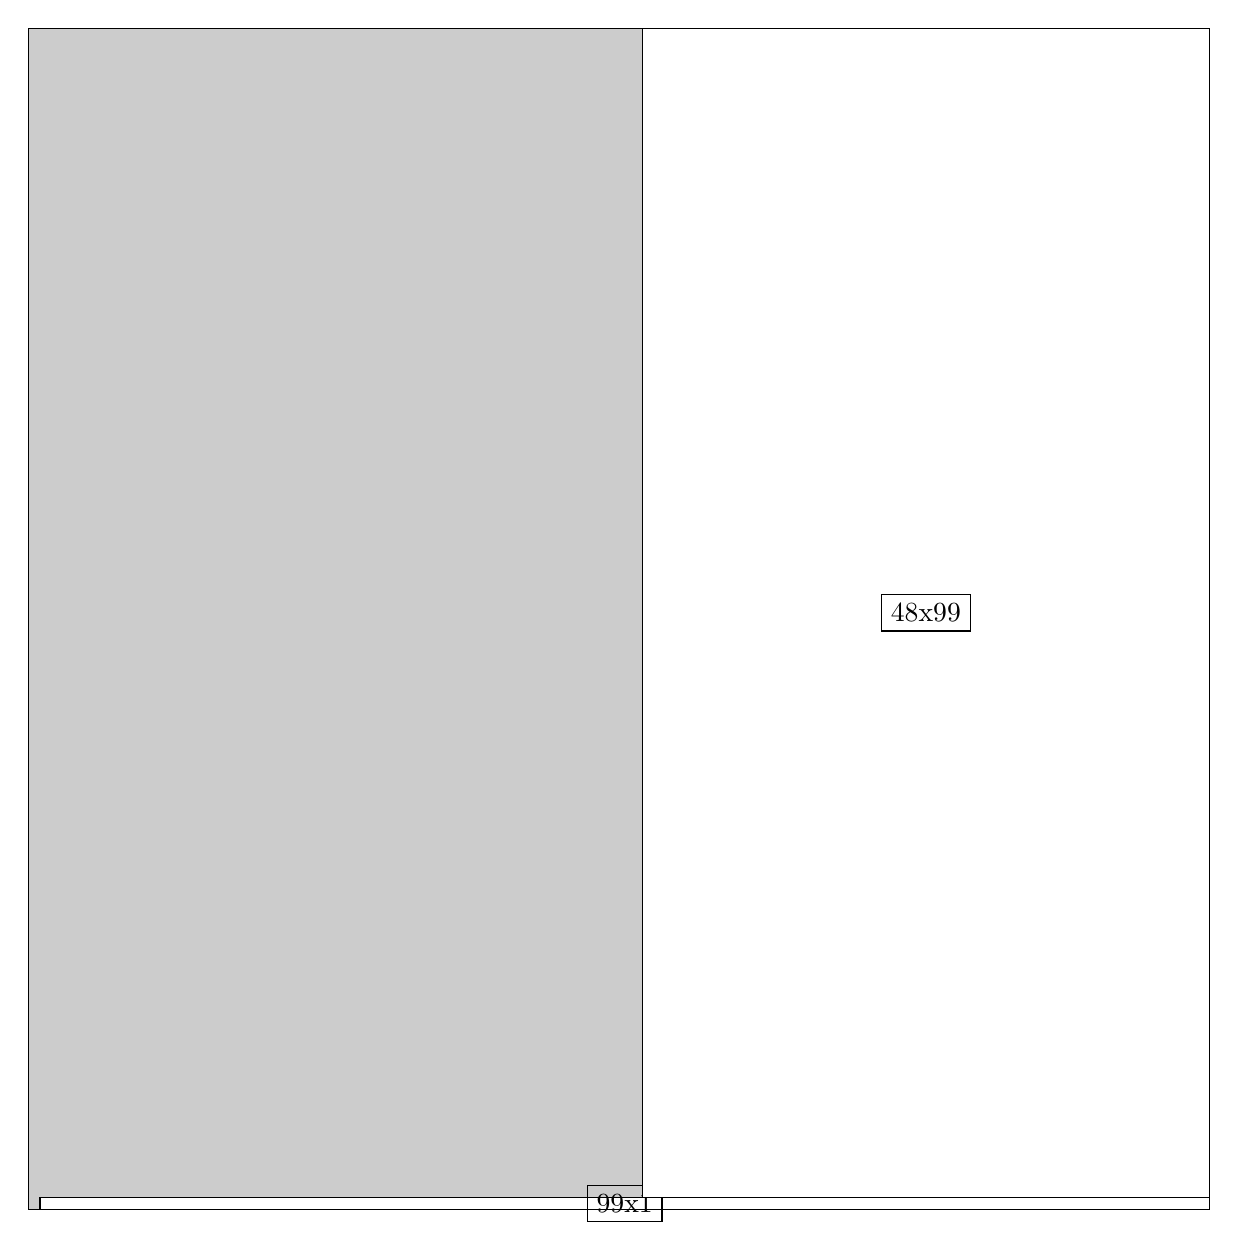
\begin{tikzpicture}[shorten >=1pt,scale=1.0,every node/.style={scale=1.0},->]
\tikzstyle{vertex}=[circle,fill=black!25,minimum size=14pt,inner sep=0pt]
\filldraw[fill=gray!40!white, draw=black] (0,0) rectangle (15.0,15.0);
\foreach \name/\x/\y/\w/\h in {99x1/0.15/0.0/14.85/0.15,48x99/7.8/0.15/7.199999999999999/14.85}
\filldraw[fill=white!40!white, draw=black] (\x,\y) rectangle node[draw] (\name) {\name} ++(\w,\h);
\end{tikzpicture}


w =99 , h =1 , x =1 , y =0 , v =99
\par
w =48 , h =99 , x =52 , y =1 , v =4752
\par
\newpage


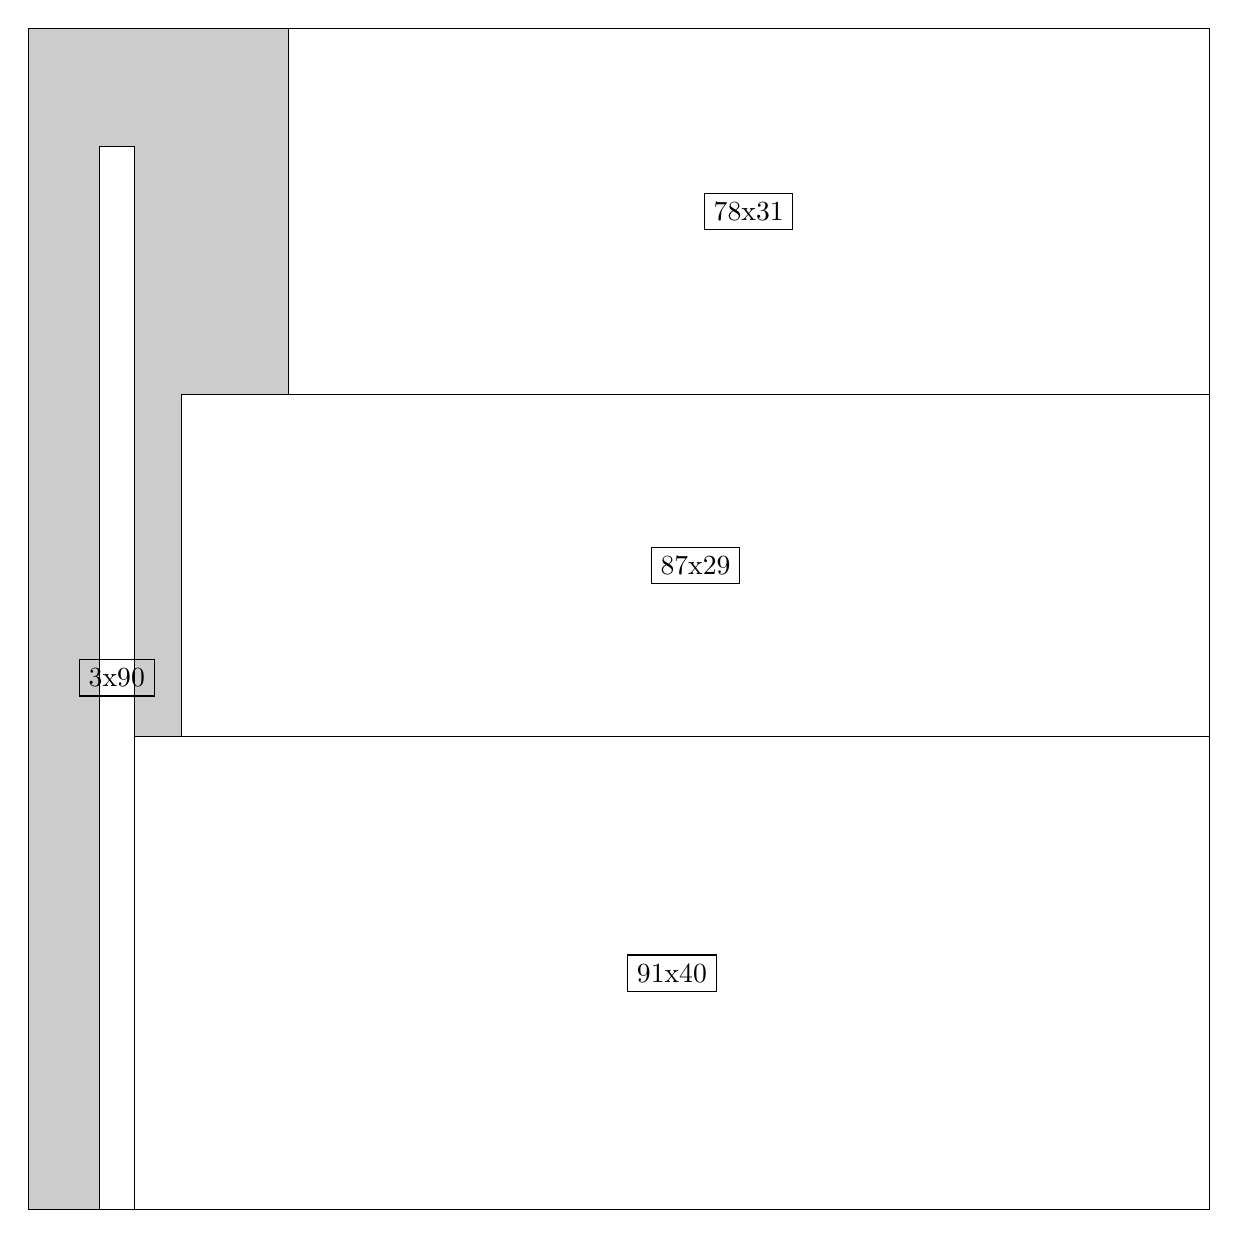
\begin{tikzpicture}[shorten >=1pt,scale=1.0,every node/.style={scale=1.0},->]
\tikzstyle{vertex}=[circle,fill=black!25,minimum size=14pt,inner sep=0pt]
\filldraw[fill=gray!40!white, draw=black] (0,0) rectangle (15.0,15.0);
\foreach \name/\x/\y/\w/\h in {91x40/1.3499999999999999/0.0/13.65/6.0,87x29/1.95/6.0/13.049999999999999/4.35,78x31/3.3/10.35/11.7/4.6499999999999995,3x90/0.8999999999999999/0.0/0.44999999999999996/13.5}
\filldraw[fill=white!40!white, draw=black] (\x,\y) rectangle node[draw] (\name) {\name} ++(\w,\h);
\end{tikzpicture}


w =91 , h =40 , x =9 , y =0 , v =3640
\par
w =87 , h =29 , x =13 , y =40 , v =2523
\par
w =78 , h =31 , x =22 , y =69 , v =2418
\par
w =3 , h =90 , x =6 , y =0 , v =270
\par
\newpage


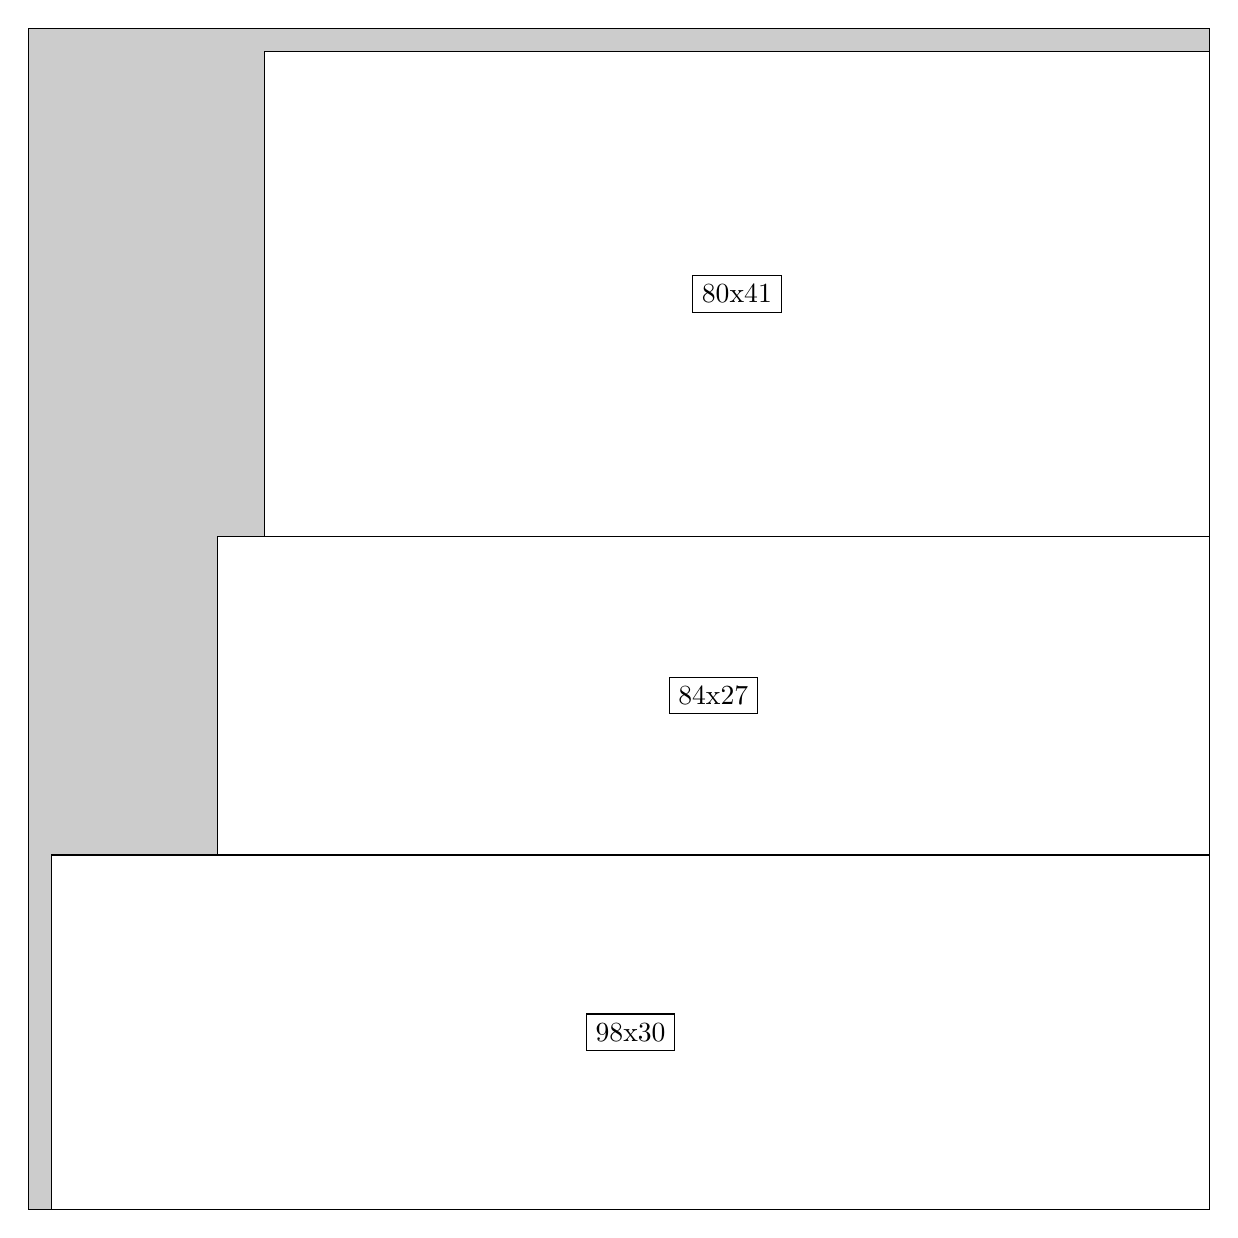
\begin{tikzpicture}[shorten >=1pt,scale=1.0,every node/.style={scale=1.0},->]
\tikzstyle{vertex}=[circle,fill=black!25,minimum size=14pt,inner sep=0pt]
\filldraw[fill=gray!40!white, draw=black] (0,0) rectangle (15.0,15.0);
\foreach \name/\x/\y/\w/\h in {98x30/0.3/0.0/14.7/4.5,84x27/2.4/4.5/12.6/4.05,80x41/3.0/8.549999999999999/12.0/6.1499999999999995}
\filldraw[fill=white!40!white, draw=black] (\x,\y) rectangle node[draw] (\name) {\name} ++(\w,\h);
\end{tikzpicture}


w =98 , h =30 , x =2 , y =0 , v =2940
\par
w =84 , h =27 , x =16 , y =30 , v =2268
\par
w =80 , h =41 , x =20 , y =57 , v =3280
\par
\newpage


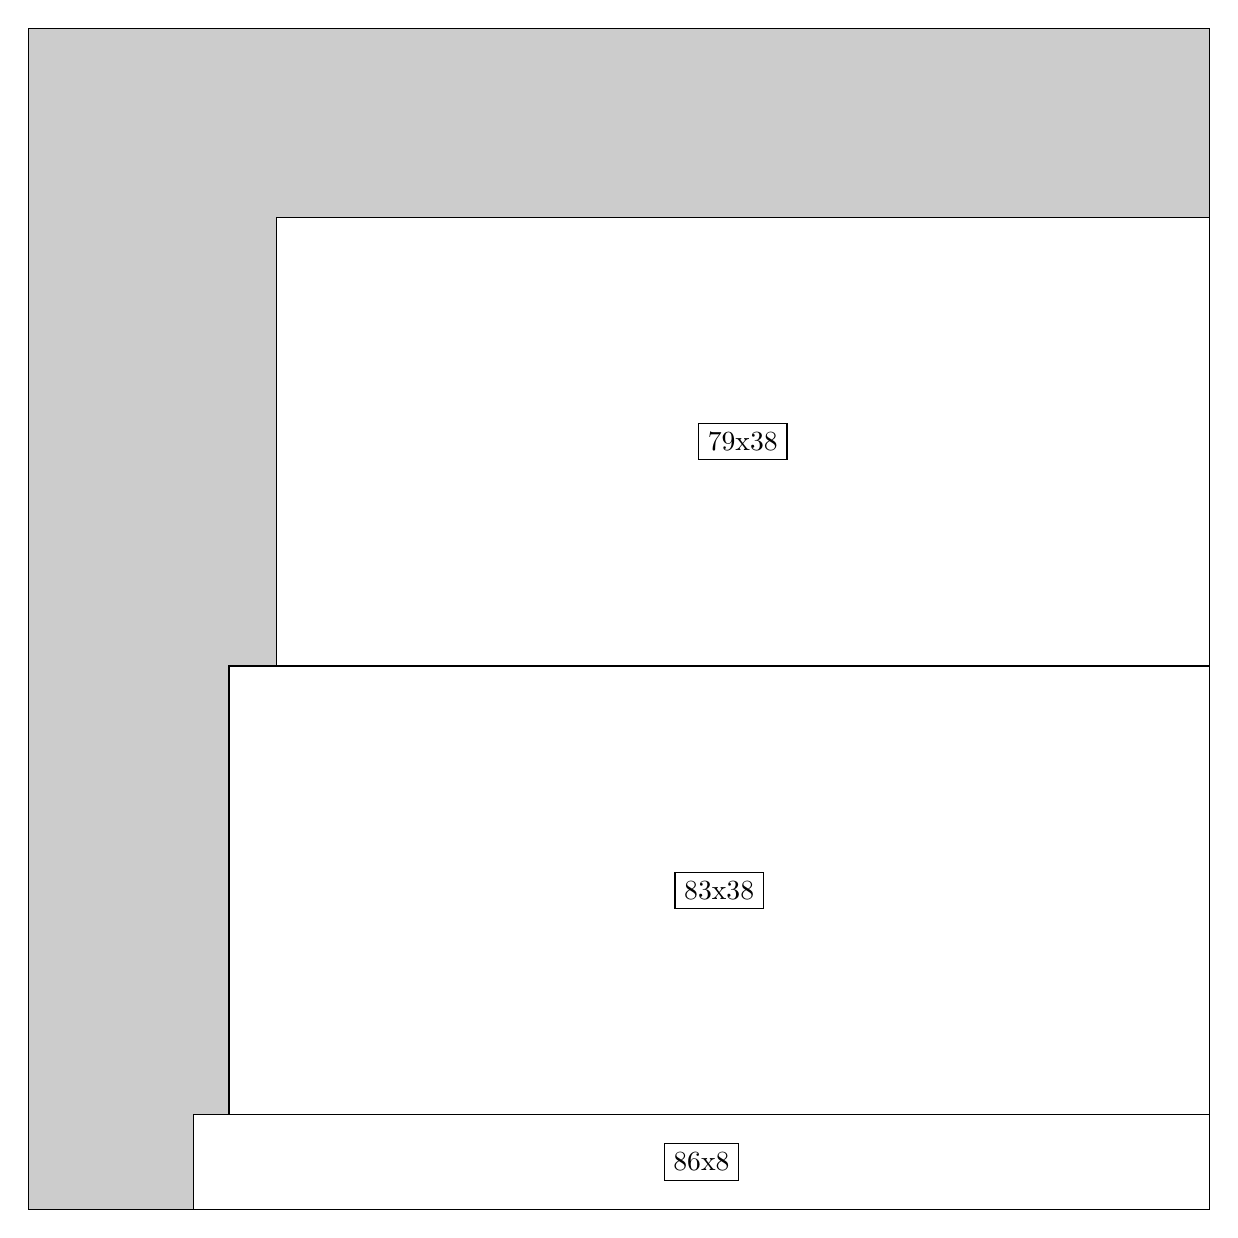
\begin{tikzpicture}[shorten >=1pt,scale=1.0,every node/.style={scale=1.0},->]
\tikzstyle{vertex}=[circle,fill=black!25,minimum size=14pt,inner sep=0pt]
\filldraw[fill=gray!40!white, draw=black] (0,0) rectangle (15.0,15.0);
\foreach \name/\x/\y/\w/\h in {86x8/2.1/0.0/12.9/1.2,83x38/2.55/1.2/12.45/5.7,79x38/3.15/6.8999999999999995/11.85/5.7}
\filldraw[fill=white!40!white, draw=black] (\x,\y) rectangle node[draw] (\name) {\name} ++(\w,\h);
\end{tikzpicture}


w =86 , h =8 , x =14 , y =0 , v =688
\par
w =83 , h =38 , x =17 , y =8 , v =3154
\par
w =79 , h =38 , x =21 , y =46 , v =3002
\par
\newpage


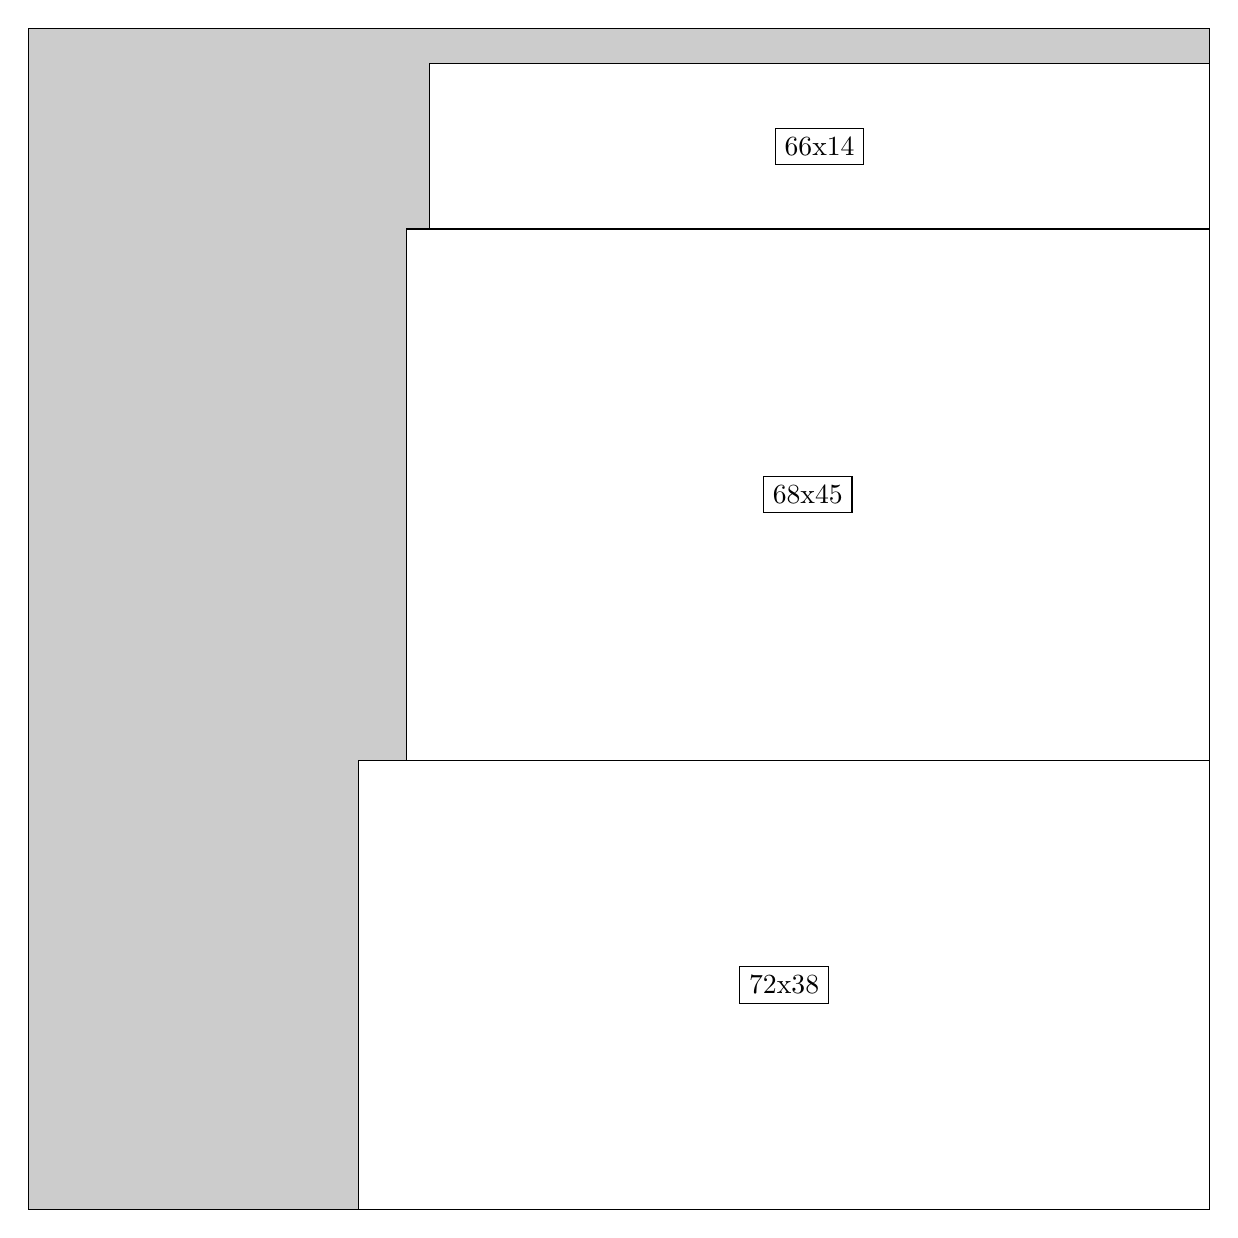
\begin{tikzpicture}[shorten >=1pt,scale=1.0,every node/.style={scale=1.0},->]
\tikzstyle{vertex}=[circle,fill=black!25,minimum size=14pt,inner sep=0pt]
\filldraw[fill=gray!40!white, draw=black] (0,0) rectangle (15.0,15.0);
\foreach \name/\x/\y/\w/\h in {72x38/4.2/0.0/10.799999999999999/5.7,68x45/4.8/5.7/10.2/6.75,66x14/5.1/12.45/9.9/2.1}
\filldraw[fill=white!40!white, draw=black] (\x,\y) rectangle node[draw] (\name) {\name} ++(\w,\h);
\end{tikzpicture}


w =72 , h =38 , x =28 , y =0 , v =2736
\par
w =68 , h =45 , x =32 , y =38 , v =3060
\par
w =66 , h =14 , x =34 , y =83 , v =924
\par
\newpage


\end{document}